%%%%%%%%%%%%%%%%%%%%%%%% ExtendedAbstract.tex %%%%%%%%%%%%%%%%%%%%%%%%
%                                                                    %
%  Template for the 10-page extended abstract to be submitted for    %
%  the MSc degree conferral at Instituto Superior Tecnico.           %
%                                                                    %
%  Author:                                                           %
%                                                                    %
%       Andre C. Marta                                               %
%       Area Cientifica de Mecanica Aplicada e Aeroespacial          %
%       Departamento de Engenharia Mecanica                          %
%       Instituto Superior Tecnico                                   %
%       Av. Rovisco Pais                                             %
%       1049-001 Lisboa                                              %
%       Portugal                                                     %
%       Tel: +351 21 841 9466                                        %
%                        3466 (extension)                            %
%       Email: andre.marta@ist.utl.pt                                %
%                                                                    %
%  Created:       Dec  2, 2011                                       %
%  Last Modified: Dec 27, 2011                                       %
%%%%%%%%%%%%%%%%%%%%%%%%%%%%%%%%%%%%%%%%%%%%%%%%%%%%%%%%%%%%%%%%%%%%%%
% This document uses the LaTeX class file "article.cls"              %
%%%%%%%%%%%%%%%%%%%%%%%%%%%%%%%%%%%%%%%%%%%%%%%%%%%%%%%%%%%%%%%%%%%%%%
\documentclass[10pt,a4paper,twocolumn]{article}

%%%%%%%%%%%%%%%%%%%%%%%%%%%%%%%%%%%%%%%%%%%%%%%%%%%%%%%%%%%%%%%%%%%%%%
% Document preamble
%%%%%%%%%%%%%%%%%%%%%%%%%%%%%%%%%%%%%%%%%%%%%%%%%%%%%%%%%%%%%%%%%%%%%%
%% Builds upon the graphics  package, providing a key-value interface
%% for optional arguments to the \includegraphics command that go far
%% beyone what the graphics package offers.
%% http://www.ctan.org/tex-archive/help/Catalogue/entries/graphicx.html
%% if you use PostScript figures in your article
%% use the graphics package for simple commands
%% \usepackage{graphics}
%% or use the graphicx package for more complicated commands
%% \usepackage{graphicx}
%% or use the epsfig package if you prefer to use the old commands
%% \usepackage{epsfig}
\usepackage{graphicx} % Enhanced LaTeX Graphics

% Multiple figures
\usepackage{subfigure} % subcaptions for subfigures
\usepackage{subfigmat} % matrices of similar subfigures

% Declaring new column types
% 'dcolumn' package defines D to be a column specifier with
% three arguments: D{<sep.tex>}{<sep.dvi>}{<decimal places>}
%                  D{<sep.tex>}{<sep.dvi>}{<left digit places>.<right digit places>}
\usepackage{dcolumn}           % decimal-aligned tabular math columns
% d takes a single argument specifying the number of decimal places, e.g., d{2}
% or the number of digits to the left and right of the seperator, e.g., d{3.2}
\newcolumntype{.}   {D{.}{.}{-1}} % column alignedd on the point separator '.'
\newcolumntype{d}[1]{D{.}{.}{#1}} % column centered on the point separator '.'
\newcolumntype{e}   {D{E}{E}{-1}} % column centered on the exponent 'E'
\newcolumntype{E}[1]{D{E}{E}{#1}} % column centered on the exponent 'E'

%% American Mathematical Society (AMS) plain Tex macros
%%
%% The amsmath package is the principal package in the AMS-LaTeX distribution
%% http://www.ctan.org/tex-archive/help/Catalogue/entries/amsmath.html
\usepackage{amsmath}
%%
%% The amsfonts package provides extended TeX fonts
%% http://www.ctan.org/tex-archive/help/Catalogue/entries/amsfonts.html
\usepackage{amsfonts}
%% The amssymb package provides various useful mathematical symbols
\usepackage{amssymb}
%%
%% The amsthm package provides extended theorem environments
%% http://www.ctan.org/tex-archive/help/Catalogue/entries/amsthm.html
\usepackage{amsthm}

%% Improves the interface for defining floating objects such as figures and tables.
%% The package also provides the H float modifier option of the obsolete here package.
%% http://www.ctan.org/tex-archive/help/Catalogue/entries/float.html
\usepackage{float}

%% Control sectional headers. 
%% http://www.ctan.org/tex-archive/help/Catalogue/entries/sectsty.html
\usepackage{sectsty}
%%
%% Redefine the font size of the 'section' and 'subsection' headings
\newcommand{\myFontSize}{\fontsize{10}{0}\selectfont}
\sectionfont{\myFontSize}       % 10pt, Bold face (default)
\subsectionfont{\rm\myFontSize} % 10pt, Plain face
\subsubsectionfont{\rm\myFontSize} % 10pt, Plain face

%% Select alternative section titles.
%% http://www.ctan.org/tex-archive/help/Catalogue/entries/titlesec.html
\usepackage{titlesec}
%%
%% Left indent, before and after spacing
%% (The starred version kills the indentation of the paragraph following the title)
\titlespacing*{\section}{0pt}{10pt}{0pt}
\titlespacing*{\subsection}{0pt}{10pt}{0pt}
\titlespacing*{\subsubsection}{0pt}{0pt}{0pt}

%% Section numbers with trailing dots. 
%% http://www.ctan.org/tex-archive/help/Catalogue/entries/secdot.html
\usepackage{secdot}
%%
%% Also put a dot after the subsection number
\sectiondot{subsection}
\sectiondot{subsubsection}
%% Set a space between dot and heading text
\sectionpunct{section}{. }    % By default, \sectiondot places a \quad
\sectionpunct{subsection}{. } % after the number
\sectionpunct{subsubsection}{. } % after the number

% These are exact settings for a A4 page with top margin of
% 25 mm, bottom margin of 30 mm, left and right margins of 25 mm,
% printable area 242 X 160 mm.

\setlength{\topmargin}{-10.4mm}
\setlength{\headheight}{0.0mm}
\setlength{\headsep}{10.0mm}
\setlength{\textwidth}{160mm}
\setlength{\textheight}{242mm}
\setlength{\oddsidemargin}{0mm}
\setlength{\evensidemargin}{0mm}
\setlength{\marginparwidth}{0mm}
\setlength{\marginparsep}{0mm}

% New command to refer to equations as Eq.(1),Eq.(2),...
\newcommand{\eqnref}[1]{Eq.(\ref{#1})}


\usepackage{eurosym}
\graphicspath{ {../Thesis_Text/Figures/} }
\usepackage[pdftex]{hyperref}
\renewcommand*{\figureautorefname}{Figure}
\renewcommand*{\tableautorefname}{Table}
\usepackage[square]{natbib} 
\usepackage{siunitx}
\DeclareSIUnit\year{yr}
\DeclareSIUnit\EUR{\text{\euro}}
\usepackage{epsfig}
\usepackage{color,soul}
\usepackage{physics}
\usepackage{makecell}
\usepackage{bbm}
\usepackage{multirow}
\usepackage[utf8]{inputenc}
\usepackage{mathtools}
\usepackage{booktabs}
\usepackage{cuted}
\usepackage{multicol}
\newlength\wttlinewidth
\setlength{\wttlinewidth}{0.4pt}
\setlength\tabcolsep{4pt}
\newenvironment{strip2}{\begin{strip}\vspace{-15pt}
\hrule width \dimexpr(0.5\textwidth-0.5\columnsep-0.4pt) \relax}{\hfill\rule[0.5\baselineskip]{\dimexpr(0.5\textwidth-0.5\columnsep-1pt)}{\wttlinewidth}
\vspace{-15pt}\end{strip}}


%%%%%%%%%%%%%%%%%%%%%%%%%%%%%%%%%%%%%%%%%%%%%%%%%%%%%%%%%%%%%%%%%%%%%%%%%%%%%%%%%%%%%%%%
% Title, authors and addresses

\title{Volatility Models in Option Pricing}
\date{Month 2018}
\author{Miguel Ribeiro \\ miguel.a.ribeiro@tecnico.ulisboa.pt \\ \\ Instituto Superior T\'{e}cnico, Lisboa, Portugal}

%%%%%%%%%%%%%%%%%%%%%%%%%%%%%%%%%%%%%%%%%%%%%%%%%%%%%%%%%%%%%%%%%%%%%%%%%%%%%%%%%%%%%%%%
\begin{document}

% Begin one column section for title and abstract
%
% http://www.faqs.org/faqs/de-tex-faq/part5/
\twocolumn[
\begin{@twocolumnfalse}
\maketitle

%%%%%%%%%%%%%%%%%%%%%%%%%%%%%%%%%%%%%%%%%%%%%%%%%%%%%%%%%%%%%%%%%%%%%%
% ABSTRACT & KEYWORDS
%%%%%%%%%%%%%%%%%%%%%%%%%%%%%%%%%%%%%%%%%%%%%%%%%%%%%%%%%%%%%%%%%%%%%%
%%%%%%%%%%%%%%%%%%%%%%%%%%%%%%%%%%%%%%%%%%%%%%%%%%%%%%%%%%%%%%%%%%%%%%
%     File: ExtendedAbstract_abstr.tex                               %
%     Tex Master: ExtendedAbstract.tex                               %
%                                                                    %
%     Author: Andre Calado Marta                                     %
%     Last modified : 2 Dez 2011                                     %
%%%%%%%%%%%%%%%%%%%%%%%%%%%%%%%%%%%%%%%%%%%%%%%%%%%%%%%%%%%%%%%%%%%%%%
% The abstract of should have less than 500 words.
% The keywords should be typed here (three to five keywords).
%%%%%%%%%%%%%%%%%%%%%%%%%%%%%%%%%%%%%%%%%%%%%%%%%%%%%%%%%%%%%%%%%%%%%%

%%
%% Abstract
%%
\begin{abstract}

Volatility is one of the most important subjects in all of quantitative finance, due not only to its impact on the prices of options but also to its elusiveness. In this thesis we study some of the models most used to forecast this variable, namely Dupire's local volatility as well as Heston and Static/Dynamic SABR stochastic volatility models.
We train these models with some options' implied volatility data, making them able to replicate real market behavior. We find that, when dealing with options with a single maturity, the Static SABR model is the one that best fits the data, while with multiple maturities, the Heston model outperforms Dynamic SABR. All these models vastly outperform the constant volatility model, assumed in Black-Scholes.
We then use these trained models to price European and Barrier options with the Monte Carlo numerical pricing method, which is able to accurately predict implied volatilities for near-the-money options, failing for deep in-the-money European call options.
\\
%%
%% Keywords (max 5)
%%
\noindent{{\bf Keywords:}} Volatility, Option pricing, Dupire, Heston, Static SABR, Dynamic SABR \\

\end{abstract}



% End one column section (begin default two columns)
\end{@twocolumnfalse}
]
%%%%%%%%%%%%%%%%%%%%%%%%%%%%%%%%%%%%%%%%%%%%%%%%%%%%%%%%%%%%%%%%%%%%%%
% INTRODUCTION
%%%%%%%%%%%%%%%%%%%%%%%%%%%%%%%%%%%%%%%%%%%%%%%%%%%%%%%%%%%%%%%%%%%%%%
%%%%%%%%%%%%%%%%%%%%%%%%%%%%%%%%%%%%%%%%%%%%%%%%%%%%%%%%%%%%%%%%%%%%%%
%     File: ExtendedAbstract_intro.tex                               %
%     Tex Master: ExtendedAbstract.tex                               %
%                                                                    %
%     Author: Andre Calado Marta                                     %
%     Last modified : 27 Dez 2011                                    %
%%%%%%%%%%%%%%%%%%%%%%%%%%%%%%%%%%%%%%%%%%%%%%%%%%%%%%%%%%%%%%%%%%%%%%
% State the objectives of the work and provide an adequate background,
% avoiding a detailed literature survey or a summary of the results.
%%%%%%%%%%%%%%%%%%%%%%%%%%%%%%%%%%%%%%%%%%%%%%%%%%%%%%%%%%%%%%%%%%%%%%

\section{Introduction}
\label{sec:intro}
Derivatives are currently one of the most studied subjects in all of mathematical finance.
In finance, a \emph{derivative} is simply a contract whose value depends on other simpler financial instruments, known as \emph{underlying assets}, such as stock prices or interest rates. These contracts are currently responsible for over \textdollar542 trillion worth of trades, in the Over-the-Counter (OTC) market alone~\citep{BIS}.
We can thus see that fully understanding the behavior of derivatives is crucial to investors.


\subsection{Options}
Of all classes of derivatives, in this master thesis we focus particularly on the most traded type~\citep{Hull}: \emph{options}.
A (European) \emph{option} contract grants its buyer the \emph{option} to buy (in the case of a \emph{call} type option) or sell (for \emph{put} options) its underlying asset, referred to as \emph{stock}, at a future date, known as the \emph{maturity}, for a fixed price, known as the \emph{strike price}.
There are other option types, such as \emph{Barrier options}, that behave similarly to European options with the condition that they only become valid if the stock price increases past a given threshold at any point until the maturity.


It's important to emphasize the fact that an option grants its buyer the \emph{right} to do something. If \emph{exercising} the option would lead to losses, the buyer can simply decide to let the maturity date pass, allowing the option to expire without further losses.

Due to their importance, finding the ideal price of an option is a major concern to investors, though this can be very difficult for some option types.

\subsection{Volatility}
Volatility is a parameter that is used in all pricing models and that greatly affects option prices. Despite its importance and our great efforts to study it, this parameter remains as one of the most elusive phenomena in all of quantitative finance, mainly due to our inability not only to forecast its behavior but even actually to accurately measure it.

Many models have been developed throughout the years in an attempt to model this parameter, with varying degrees of success. We will analyze in detail some of the most famous ones, comparing them with one another.




%%%%%%%%%%%%%%%%%%%%%%%%%%%%%%%%%%%%%%%%%%%%%%%%%%%%%%%%%%%%%%%%%%%%%%
% BACKGROUND
%%%%%%%%%%%%%%%%%%%%%%%%%%%%%%%%%%%%%%%%%%%%%%%%%%%%%%%%%%%%%%%%%%%%%%
%%%%%%%%%%%%%%%%%%%%%%%%%%%%%%%%%%%%%%%%%%%%%%%%%%%%%%%%%%%%%%%%%%%%%%
%     File: ExtendedAbstract_backg.tex                               %
%     Tex Master: ExtendedAbstract.tex                               %
%                                                                    %
%     Author: Andre Calado Marta                                     %
%     Last modified : 27 Dez 2011                                    %
%%%%%%%%%%%%%%%%%%%%%%%%%%%%%%%%%%%%%%%%%%%%%%%%%%%%%%%%%%%%%%%%%%%%%%
% A Theory section should extend, not repeat, the background to the
% article already dealt with in the Introduction and lay the
% foundation for further work.
%%%%%%%%%%%%%%%%%%%%%%%%%%%%%%%%%%%%%%%%%%%%%%%%%%%%%%%%%%%%%%%%%%%%%%

\section{Background}
\label{sec:backg}
We begin by providing some of the financial background required to understand the later results.

\subsection{Option payoffs and prices}
From the definition of a European option we can deduce the payoff function of this contract as
\begin{subequations}\label{callput}
\begin{align}
&\text{Payoff}_{Euro,\ call}(K,T)=\max\left(S(T)-K,0\right);\\
&\text{Payoff}_{Euro,\ put}(K,T)=\max\left(K-S(T),0\right),
\end{align}
\end{subequations}
\noindent where $K$ is the option's strike price and $S(T)$ is the asset's price, $S(t)$, at the maturity, $T$.


An up-and-in Barrier option's payoff function is exactly as shown in eq.\eqref{callput} conditioned on a given threshold $B$ being surpassed at any point until the maturity (i.e. $\exists\,t<T\,:\,S(t)>B$). It should be zero otherwise.
The influence of this threshold $B$ on the option price is trivial: because it is linked to the probability of the stock price reaching $B$, the higher the barrier $B$, the lower the corresponding option price.

We can price options by setting their expected profit to be the same as a risk-neutral investment, (e.g. bank deposit). The price of an option can thus be deduced as it's expected future payoff, discounted back to the present
\begin{equation}\label{pricepayoff}
\text{Price}(K,T)=e^{-rT}\mathbb{E}\left[\text{Payoff}(K,T)\right],
\end{equation}
\noindent where $r$ is the risk-free interest rate, defined as the interest an investor would receive from any risk-free investment (e.g. treasury bills). In general, this rate changes slightly with time and is unknown.

\subsection{Black-Scholes Formulae}
Fischer Black and Myron Scholes developed a mathematical model to price European options - the famous Black-Scholes (BS) model~\citep{Scholes} - still in use in present days~\citep{Wilmott3}.

This model states that the price of a European option follows the partial differential equation
\begin{equation}\label{BS2}
\pdv{V}{t}+\frac{1}{2}\sigma^2S^2\pdv{^2V}{S^2}+rS\pdv{V}{S}-rV=0,
\end{equation}
\noindent where $V$ is the price of the option and $\sigma$ is the stock price volatility, which affects how erratically the stock price moves. The interest rate, $r$, is assumed to be a known function of time, and the volatility, $\sigma$, is assumed to be a known constant.

Under this model, we assume that stock prices follow a Geometric Brownian Motion (GBM), defined as
\begin{equation}\label{GBM}
dS(t)=rS(t)dt+\sigma S(t)dW(t),
\end{equation}
\noindent with $\{W(t),\ t>0\}$ defining a one-dimensional Brownian motion. An example of such processes is represented in \autoref{fig:GBM}.

\begin{figure}[H]
    \centering
      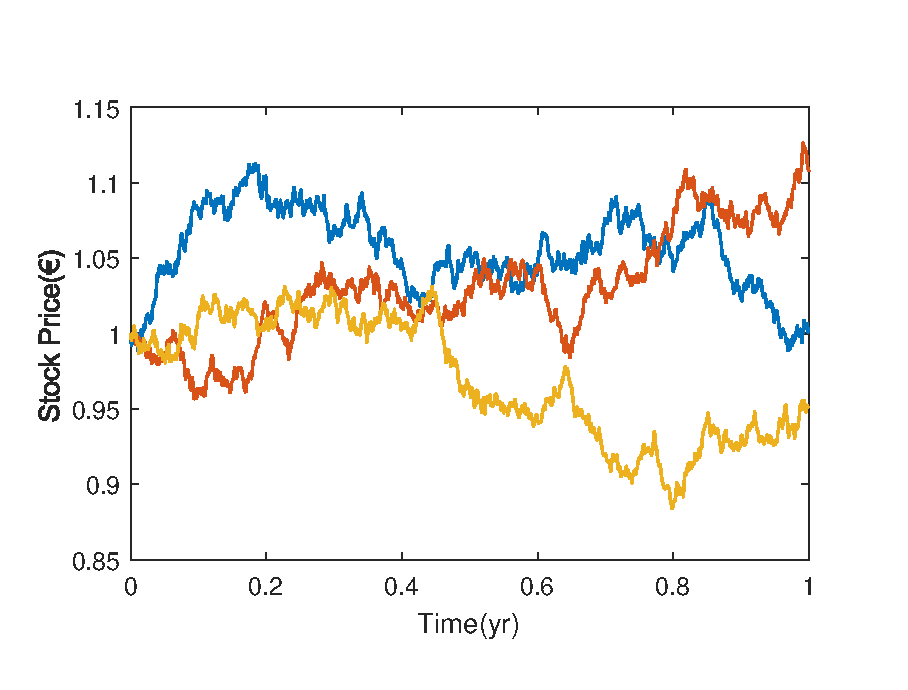
\includegraphics[width=.8\columnwidth,trim={0.35cm 0.6cm 1.4cm 1.35cm},clip]{GBM.eps}
      \caption{Example of three Geometric Brownian Motion processes.}\label{fig:GBM}
    \end{figure}
    
To price options, we need to solve the PDE in eq.\eqref{BS2} as we would for the diffusion equation's initial value problem~\citep{Dilao}, resulting in
\begin{subequations}\label{callputBS}
\begin{align}
&C(K,T)=N(d_1)S_0-N(d_2)Ke^{-rT};\\
&P(K,T)=-N(-d_1)S_0+N(-d_2)Ke^{-rT},
\end{align}
\end{subequations}
\noindent where $N(\cdot)$ is the cumulative distribution function of the standard normal distribution and where $d_1$, $d_2$ are given by
\begin{subequations}\label{d1d2}
\begin{align}
&d_1=\frac{1}{\sigma\sqrt{T}}\left[\log\left(\frac{S_0}{K}\right)+\left(r+\frac{\sigma^2}{2}\right)T\right];\\
&d_2=d_1-\sigma\sqrt{T}.
\end{align}
\end{subequations}


In \autoref{fig:Inception} we represent the values of call and put options at both the inception (i.e. $t=0$) and maturity.
\begin{figure}[H]
    \centering
      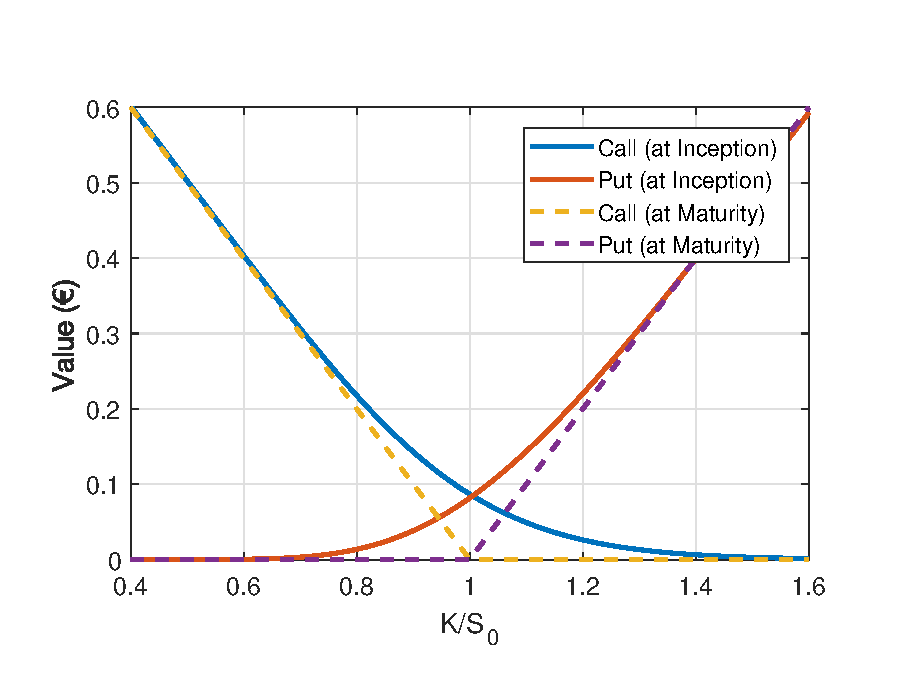
\includegraphics[width=.8\columnwidth,trim={0.6cm 0.4cm 1.15cm 1.4cm},clip]{Inception.eps}
      \caption{Call and Put option values at inception and maturity}\label{fig:Inception}
    \end{figure}

We can thus use eqs.\eqref{callputBS} to precisely price European options, so long as all the parameters are exactly known and remain constant throughout the option's duration (which is never true).

%%%%%%%%%%%%%%%%%%%%%%%%%%%%%%%%%%%%%%%%%%%%%%%%%%%%%%%%%%%%%%%%%%%%%%
%     File: ExtendedAbstract_concl.tex                               %
%     Tex Master: ExtendedAbstract.tex                               %
%                                                                    %
%     Author: Andre Calado Marta                                     %
%     Last modified : 27 Dez 2011                                    %
%%%%%%%%%%%%%%%%%%%%%%%%%%%%%%%%%%%%%%%%%%%%%%%%%%%%%%%%%%%%%%%%%%%%%%
% The main conclusions of the study presented in short form.
%%%%%%%%%%%%%%%%%%%%%%%%%%%%%%%%%%%%%%%%%%%%%%%%%%%%%%%%%%%%%%%%%%%%%%

\section{Volatility}
\label{sec:vol}
Volatility is a measure of the uncertainty in future stock price movements - a higher volatility will lead to greater future fluctuations in the stock price, whereas a stock with lower volatility is more stable. This influence is represented in \autoref{fig:VarVol}.
\begin{figure}[H]
    \centering
      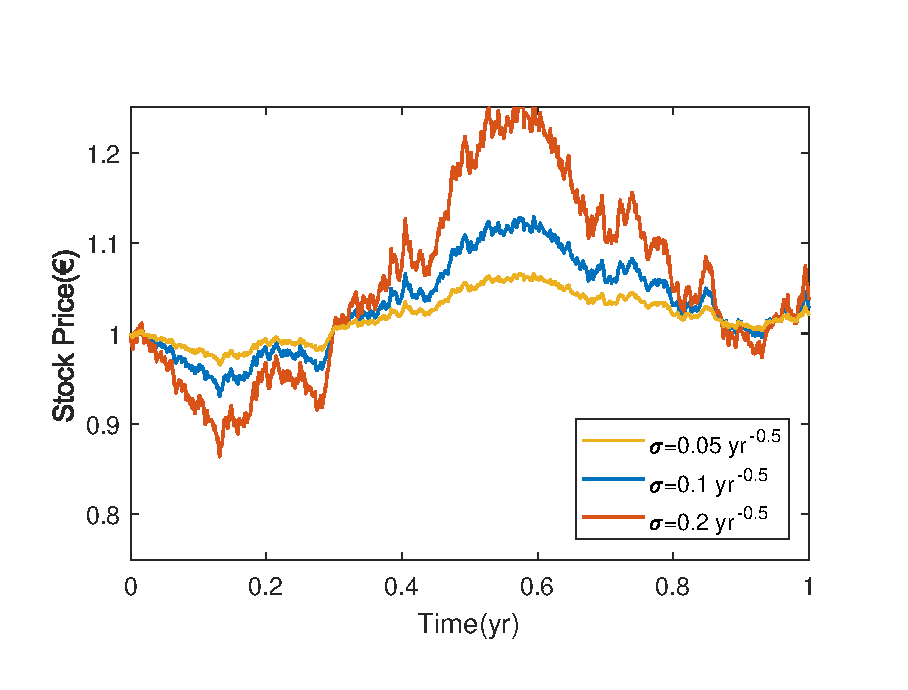
\includegraphics[width=.8\columnwidth,trim={0.6cm 0.55cm 1.35cm 1.5cm},clip]{VarVol.eps}
      \caption{Example of three realizations of GBM processes with different volatilities}\label{fig:VarVol}
    \end{figure}
    
Of all the parameters in the BS model, volatility is the only one we can't easily estimate or predict, even though it has a major impact on the prices of options.

It is usually estimated empirically from the standard deviation of the historical rate of log-returns~\citep{Hull}, defined as
\begin{equation}
s=\sqrt{\frac{1}{n-1}\sum_{i=1}^n(u_i-\overline{u})^2},
\end{equation}
\noindent where the log-return rate, $u_i$, is given by
\begin{equation}
u_i=\log\left(\frac{S_i}{S_{i-1}}\right),
\end{equation}
\noindent with $\overline{u}$ defining its average and $S_i$ corresponding to the stock price at the $i$\textsuperscript{th} measurement of some given set of past observations.


Using this result, we are able to estimate the volatility of any given asset at the present moment and use it in the BS model, if we assume it remains constant in the future. The clear problem with this approach is that, when observing market data, we can see that \emph{volatilities change over time}~\citep{chourdakis}. \emph{If we try to price options assuming a constant volatility, our options will become mispriced, causing potential losses}.

Our goal is to model the instantaneous volatility (i.e. the volatility at a given point in time) and, with this model, predict its future behavior, using this knowledge to better price options.
Many models have been developed in the past, so we will only study some of the most used ones, namely Dupire's formula, where we assume that the volatility depends on the stock price and time (i.e. $\sigma=\sigma(t,S(t))$), and three other models, Heston and Static/Dynamic SABR, where the volatility itself is assumed to be a stochastic process (i.e. $\sigma=\sigma(t,S(t),W(t))$).

\subsection{Implied Volatility}
To fully understand the results shown next we need the concept of implied volatility.
\emph{Implied volatility} can be defined as the value of stock price volatility that, when input into the BS pricer in eq.\eqref{callputBS}, outputs a price equal to the market price of a given option.

Because eq.\eqref{callputBS} is not explicitly invertible w.r.t. $\sigma$, we need to use some numerical method (e.g. Newton's method) to find the value of implied volatility that matches market with model prices, i.e. we must find, numerically, the solution to the equation
\begin{equation}\label{impvolform}
C(\sigma_{imp})=C_{\mathrm{mkt}},
\end{equation}
\noindent where $C(\sigma_{imp})$ is the BS option price using $\sigma_{imp}$ as volatility and $C_{\mathrm{mkt}}$ is the price observed in the market.

It can be shown that the relation between implied volatility and option price is a monotonous increasing function (i.e. the relationship is bijective), which means that we can obtain the implied volatility of an option from its price and vice versa~\citep{Wilmott3}. Thus, we can train our models on implied volatility data instead of using option prices, since they are equivalent.

One important property of implied volatility is that, when observing real market data, we can clearly see that it depends on the strike price, which is incompatible with the BS view (which assumes it is independent).
This phenomenon is known as the implied volatility \emph{smile} and is represented in \autoref{fig:Smile} (a \emph{skew} can also be observed for some types of underlying assets).

\begin{figure}[H]
    \centering
      \includegraphics[width=.8\columnwidth,trim={1.35cm 0.45cm 1.4cm 1.5cm},clip]{Smile.eps}
      \caption{Implied volatility smile.}\label{fig:Smile}
    \end{figure}
    
It can also be shown that the implied volatility decreases with maturity, though this relationship is harder to define.

\subsection{Option Price Sensitivity and Vega}
When studying volatilities, it's very important to consider the sensitivity of the option price to the volatility, i.e. how a small variation in the volatility of a given option affects its price. This analysis is particularly important for volatilities because there is a high uncertainty associated with this parameter and a high sensitivity might lead to severe mispricing errors.

This sensitivity is usually called \emph{Vega}, or $\mathcal{V}$, and is defined as
\begin{equation}
\mathcal{V}=\pdv{V}{\sigma},
\end{equation}
\noindent where $V$ denotes the option price.
In particular for European calls, this value can be shown to be~\citep{Hull}
\begin{equation}
\mathcal{V}=S_0\sqrt{T}N'(d_1),
\end{equation}
\noindent where $d_1$ is given in eqs.\eqref{d1d2} and $N'(\cdot)$ is the probability density function for a standard normal distribution.

Despite its usefulness, the Vega doesn't grasp the whole picture e.g. a Vega of $4$ means that an absolute change of $2$ in the volatility produces an absolute change of $8$ in the option price - we don't have any information regarding the relative change of the price (i.e. if it changed by $1\%$ or $50\%$).
As we will see shortly, this information is indeed important. We thus define the \emph{relative change} as
\begin{equation}
\mathrm{Relative\ Change}=\pdv{V}{\sigma}\frac{\sigma}{V},
\end{equation}
\noindent where now a $\mathrm{Relative\ Change}$ of $4$ implies that a change of $2\%$ in the volatility produces a variation of $8\%$ in the option price. This relationship is plotted in \autoref{fig:Vega2}, for call options, against their strike price.
\begin{figure}[H]
    \centering
      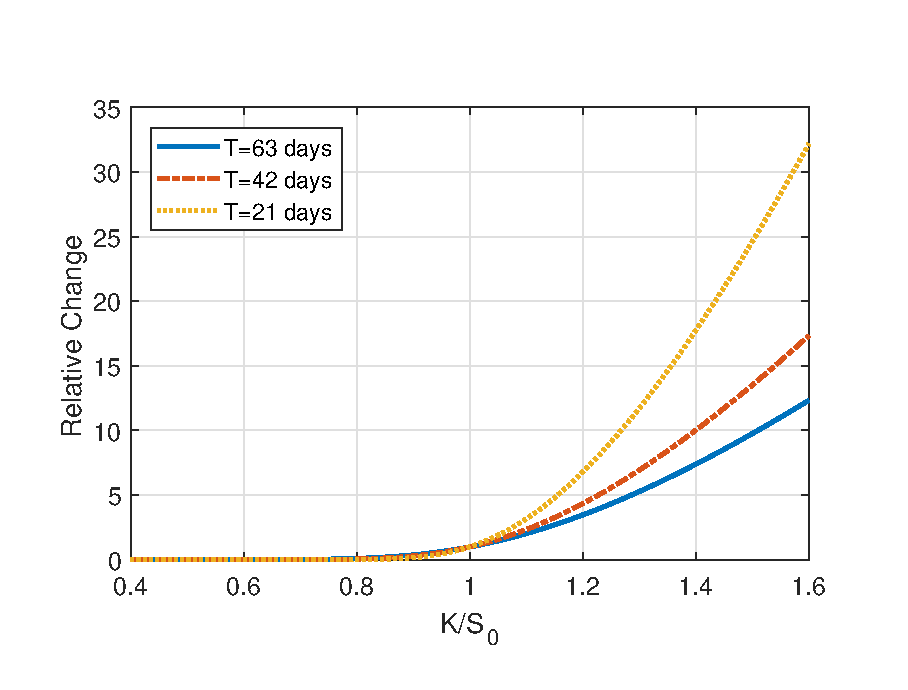
\includegraphics[width=.8\columnwidth,trim={0.7cm 0.45cm 1.1cm 1.4cm},clip]{Vega2.eps}
      \caption{Relationship between the (call) option price's relative change (w.r.t. volatility) and the respective strike prices, for different maturities.}\label{fig:Vega2}
    \end{figure}

As we can see in \autoref{fig:Vega2}, the relative change of the option price w.r.t. volatility is very large for call options with high strikes, which means that the prices of such options are very sensitive to volatility (i.e. a very slight (relative) change in the volatility will produce a very large (relative) change in the option price). It also means that the volatility is very robust w.r.t. the option price (i.e. a very large (relative) variation in the option price will barely affect the volatility).
The opposite effect is observed for call options with lower strikes, since we can see that the relative variation of the option price w.r.t. the volatility is extremely small in these cases, meaning not only that the option price is extremely robust to the volatility (i.e. a change in the volatility will barely affect the option price), but also implying that the volatility is extremely sensitive to the option price (i.e. a very slight (relative) change in the price of a call option will dramatically change its volatility).
This phenomenon will become important when we examine our results.

\subsection{Volatility Models}
As previously stated volatility not only changes with time but is also dependent on the strike price.
The (constant volatility) BS model is therefore clearly insufficient to completely grasp real-world trading and we should try to find some more appropriate volatility models.

\vspace{5pt}
\subsubsection{Dupire's Local Volatility}
One of the most used volatility models was developed by Dupire~\citep{Dupire} and uses the concept of local volatility, where we assume that volatility is a function of both time and stock price: $\sigma(S(t),t)$.
The stock price process now follows the diffusion process
\begin{equation}\label{GBM2}
dS(t)=rS(t)dt+\sigma(S(t),t)S(t)dW(t),
\end{equation}
\noindent where the local volatility, $\sigma(S(t),t)$, is a nonlinear \emph{deterministic} function of $S(t)$ and $t$.

To estimate $\sigma(S(t),t)$, we must have some implied volatility data for options with multiple strikes over multiple maturities. From this data we extract the implied volatility surface, $\sigma_{imp}(S(t),t)$, and its respective gradients w.r.t $K$ and $T$, which we can use to generate $\sigma(S(t),t)$ using

\begin{strip2}
\vspace{5pt}
\begin{equation}\label{dupire2}
\sigma(S(t),t)=\sqrt{\frac{\displaystyle\sigma_{imp}^2+2t\sigma_{imp}\pdv{\sigma_{imp}}{T}+2r(S(t))t\sigma_{imp}\pdv{\sigma_{imp}}{K}}{\displaystyle\left(1+(S(t))d_1\sqrt{t}\pdv{\sigma_{imp}}{K}\right)^2+(S(t))^2t\sigma_{imp}\left(\pdv{^2\sigma_{imp}}{K^2}-d_1\left(\pdv{\sigma_{imp}}{K}\right)^2\sqrt{t}\right)}},
\end{equation}
\end{strip2}
\noindent with $d_1$ given by
\begin{equation}
d_1=\frac{\log(S_0/S(t))+\left(r+\frac{1}{2}\sigma_{imp}^2\right)t}{\sigma_{imp}\sqrt{t}}.
\end{equation}
\noindent where we define $\sigma_{imp}=\sigma_{imp}(K,T)$ as the implied volatilities of options with maturity $T$, and strike $K$. Furthermore, $\sigma_{imp}$ and all its derivatives are evaluated at $K=S(t)$ and $T=t$.

With eq.\eqref{dupire2} we generate a local volatility surface, which we can use in eq.\eqref{GBM2} to create the respective stock price path. From this, we are able to price options, as we will see shortly.

\vspace{5pt}
\subsubsection{Heston's Stochastic Volatility}
Volatility is not constant, is not directly observable and is unpredictable. This seems to suggest that volatility is itself also a stochastic process~\citep{rebonato}.

The \emph{Heston model}, developed by Steven Heston~\citep{Heston}, is one of the most used \emph{stochastic volatility models}, and it states that stock prices satisfy the relations
\begin{equation}\label{hestons}
dS(t)=rS(t)dt+\sqrt{\nu(t)}S(t)dW_1(t),
\end{equation}
\begin{equation}\label{hestonv}
d\nu(t)=\kappa(\overline{\nu}-\nu(t))dt+\eta\sqrt{\nu(t)}dW_2(t),
\end{equation}\noindent with $\nu(t)$ corresponding to the stock price variance (i.e. the square of the volatility, $\nu(t)=(\sigma(t))^2$) and where we define $\nu_0$ as the initial variance.
Furthermore, the one-dimensional Brownian motion processes $W_1(t)$ and $W_2(t)$ have a constant correlation $\rho$, typically negative, which can be justified from market behavior~\citep{chourdakis}.

The parameters $\kappa$, $\overline{\nu}$ and $\eta$ are, respectively, the \emph{mean-reversion rate} (i.e. how fast the variance converges to its mean value), the \emph{long-term variance} (i.e. the mean value of variance) and the \emph{volatility of the variance} (i.e. how erratic is the variance process).

To appropriately use the model, we have to find the values for the parameter set $\theta=\left\{\kappa,\overline{\nu},\eta,\nu_0,\rho\right\}$ that best fit market data. For many models, this calibration process requires lengthy simulations and is impractically slow to converge. One of the reasons why the Heston model is so popular is the fact that there exists a closed-form solution that we can use to directly obtain the option prices under this model with any given parameter set $\theta$. This closed form solution (with modifications made by Schoutens~\citep{Schoutens}, Rollin \textit{et al.}~\citep{Rollin} and Cui \textit{et al.}~\citep{Cui}) is given by

\begin{strip2}
\begin{equation}\label{CH}
\begin{split}
C_{H}(K,T;\theta)&=e^{-rT}\mathbb{E}\left[\left(S(T)-K\right)\mathbbm{1}_{\left\{S(T)>K\right\}}\ \vert\ \theta\right]\\
&=e^{-rT}\left(\mathbb{E}\left[S(T)\mathbbm{1}_{\left\{S(T)>K\right\}}\ \vert\ \theta\right]-K\mathbb{E}\left[\mathbbm{1}_{\left\{S(T)>K\right\}}\ \vert\ \theta\right]\right)\\
&=S_0P_1(K,T;\theta)-e^{-rT}KP_0(K,T;\theta),
\end{split}
\end{equation}
\begin{equation}\label{P1}
P_1(K,T;\theta)=\frac{1}{2}+\frac{1}{\pi}\int_0^\infty\operatorname{Re}\left(\frac{e^{-iu\log K}}{iuS_0e^{rT}}\phi(u-i,T;\theta)\right)du,
\end{equation}
\begin{equation}\label{P2}
P_0(K,T;\theta)=\frac{1}{2}+\frac{1}{\pi}\int_0^\infty\operatorname{Re}\left(\frac{e^{-iu\log K}}{iu}\phi(u,T;\theta)\right)du,
\end{equation}
\begin{equation}
\phi(u,t;\theta)=\exp\left\{iu\left(\log S_0+rt\right)-\frac{t\kappa\overline{\nu}\rho iu}{\eta}-\nu_0A+\frac{2\kappa\overline{\nu}}{\eta^2}D\right\},
\end{equation}
\begin{equation}
D=\log \alpha+\frac{(\kappa-\alpha) t}{2}-\log\left(\frac{\alpha+\xi}{2}+\frac{\alpha-\xi}{2}e^{-\alpha t}\right),
\end{equation}
\end{strip2}
\begin{equation}
A=\frac{A_1}{A_2},
\end{equation}
\begin{equation}\label{xi}
\xi=\kappa-\eta\rho iu,
\end{equation}
\begin{equation}\label{alpha}
\alpha=\sqrt{\xi^2+\eta^2(u^2+iu)},
\end{equation}
\begin{equation}
A_1=(u^2+iu)\sinh\frac{\alpha t}{2},
\end{equation}
\begin{equation}
A_2=\alpha\cosh\frac{\alpha t}{2}+\xi\sinh\frac{\alpha t}{2}.
\end{equation}
\noindent where $C_{H}(K,T;\theta)$ corresponds to the model's European call option price, assuming a parameter set $\theta$, $i$ is the imaginary unit and where $\phi(u,t;\theta)$ is the characteristic function of the logarithm of the stock price process (the characteristic function corresponds to the Fourier transform of the probability density function of a random variable).
With this result we can easily calibrate the model by minimizing the difference between model and market prices.

\vspace{5pt}
\subsubsection{Static SABR Stochastic Volatility}
One other very commonly used stochastic volatility model was developed by Hagan \textit{et al.}~\citep{Hagan} and is known as \emph{SABR} (short for \emph{stochastic-}$\alpha\beta\rho$) (we henceforth refer to it as Static SABR to distinguish it from the Dynamic SABR model shown next). Under this model we assume that the stock price and volatility processes follow~\citep{Geeske}
\begin{equation}\label{dF}
dS(t)=rS(t)dt+e^{-r(T-t)(1-\beta)}\sigma(t)(S(t))^\beta dW_1(t),
\end{equation}
\begin{equation}\label{dsigma}
d\sigma(t)=\nu\sigma(t) dW_2(t),
\end{equation}
\noindent where $\alpha=\sigma(0)$ and, as before, the two Brownian motion processes $W_1(t)$ and $W_2(t)$ have a \emph{constant} correlation of $\rho$.

The parameters $\beta$ and $\nu$ correspond, respectively to the \emph{skewness} (i.e. how the volatility smile moves when the stock price changes) and the \emph{volatility of volatility} (i.e. how erratic is the volatility process).

As for the Heston model, in Static SABR we also have a (quasi-)closed form solution from which we can extract the option's implied volatility for any given parameter set (the respective price can be obtained with eq.\eqref{impvolform}). This formula is given by (with modifications made by Oblój~\citep{Obloj})

\newpage

\begin{strip2}
\begin{equation}\label{sabr}
\begin{split}
\sigma_{StatSABR}(K,f,T)\approx&\frac{1}{\displaystyle\left[1+\frac{(1-\beta)^2}{24}\log^2\left(\frac{f}{K}\right)+\frac{(1-\beta)^4}{1920}\log^4\left(\frac{f}{K}\right)\right]}.\left(\frac{\nu\log\left(f/K\right)}{x(z)}\right)\\
&.\left\{1+T\left[\frac{(1-\beta)^2}{24}\frac{\alpha^2}{(Kf)^{1-\beta}}+\frac{1}{4}\frac{\rho\beta\nu\alpha}{(Kf)^{(1-\beta)/2}}+\frac{2-3\rho^2}{24}\nu^2\right]\right\},
\end{split}
\end{equation}
\end{strip2}
\noindent with $z$ and $x(z)$ defined as
\begin{equation}
z=\frac{\nu\left(f^{1-\beta}-K^{1-\beta}\right)}{\alpha(1-\beta)},
\end{equation}
\begin{equation}
x(z)=\log\left\{\frac{\sqrt{1-2\rho z+z^2}+z-\rho}{1-\rho}\right\},
\end{equation}
\noindent using $f=S_0e^{rT}$.

We again need to find the optimal values for the parameters that best fit the market data.

\vspace{5pt}
\subsubsection{Dynamic SABR Stochastic Volatility}
One of the main setbacks of the Static SABR model is the fact that it behaves badly when we try to fit options with different maturities~\citep{Hagan}. To solve this, the authors developed an alternative model, known as \emph{Dynamic SABR}, similar to the Static SABR model but where we replace the parameters $\nu$ and $\rho$ with some functions of time, $\nu(t)$ and $\rho(t)$, chosen empirically.

Fernandez \textit{et al.}~\citep{Fernandez} claimed that $\nu(t)$ and $\rho(t)$ should tend to zero with time. In this work, we will use the functions suggested by those authors
\begin{equation}\label{rhot}
\rho(t)=\rho_0e^{-at},
\end{equation}
\begin{equation}\label{nut}
\nu(t)=\nu_0e^{-bt},
\end{equation}
\noindent with $\rho_0\in[-1,1]$, $\nu_0>0$, $a>0$ and $b>0$.

For this particular choice of $\nu(t)$ and $\rho(t)$, the Dynamic SABR model also has a (quasi-)closed form solution, which we can use to directly obtain the option's implied volatility with any given parameter set. This formula (with some modifications made by Osajima~\citep{Osajima}) is given by 

\begin{strip2}
\vspace{5pt}
\begin{equation}\label{dynsabr}
\sigma_{DynSABR}(K,f,T)=\frac{1}{\omega}\left(1+A_1(T)\log\left(\frac{K}{f}\right)+A_2(T)\log^2\left(\frac{K}{f}\right)+B(T)T\right),
\end{equation}
\begin{equation}
A_1(T)=\frac{\beta-1}{2}+\frac{\eta_1(T)\omega}{2},
\end{equation}
\begin{equation}
A_2(T)=\frac{(1-\beta)^2}{12}+\frac{1-\beta-\eta_1(T)\omega}{4}+\frac{4\nu_1^2(T)+3(\eta_2^2(T)-3\eta_1^2(T))}{24}\omega^2,
\end{equation}
\begin{equation}
B(T)=\frac{1}{\omega^2}\left(\frac{(1-\beta)^2}{24}+\frac{\omega\beta\eta_1(T)}{4}+\frac{2\nu_2^2(T)-3\eta_2^2(T)}{24}\omega^2\right),
\end{equation}
\begin{equation}
\nu_1^2(T)=\frac{6\nu_0^2}{(2bT)^3}\left[\left(\frac{(2bT)^2}{2}-2bT+1\right)-e^{-2bT}\right],
\end{equation}
\begin{equation}
\nu_2^2(T)=\frac{12\nu_0^2}{(2bT)^3}\left[e^{-2bT}(1+bT)+bT-1\right],
\end{equation}
\begin{equation}
\eta_1(T)=\frac{2\nu_0\rho_0}{T^2(a+b)^2}\left[(a+b)T+e^{-(a+b)T}-1\right],
\end{equation}
\begin{equation}
\eta_2^2(T)=\frac{3\nu_0^2\rho_0^2}{T^4(a+b)^4}\left[e^{-2(a+b)T}-8e^{-(a+b)T}+(7+2T(a+b)(-3+(a+b)T))\right].
\end{equation}
\end{strip2}
\noindent where $f=S_0e^{rT}$ and $\omega=f^{1-\beta}/\alpha$.

%%%%%%%%%%%%%%%%%%%%%%%%%%%%%%%%%%%%%%%%%%%%%%%%%%%%%%%%%%%%%%%%%%%%%%
% IMPLEMENTATION
%%%%%%%%%%%%%%%%%%%%%%%%%%%%%%%%%%%%%%%%%%%%%%%%%%%%%%%%%%%%%%%%%%%%%%
%%%%%%%%%%%%%%%%%%%%%%%%%%%%%%%%%%%%%%%%%%%%%%%%%%%%%%%%%%%%%%%%%%%%%%
%     File: ExtendedAbstract_imple.tex                               %
%     Tex Master: ExtendedAbstract.tex                               %
%                                                                    %
%     Author: Andre Calado Marta                                     %
%     Last modified : 27 Dez 2011                                    %
%%%%%%%%%%%%%%%%%%%%%%%%%%%%%%%%%%%%%%%%%%%%%%%%%%%%%%%%%%%%%%%%%%%%%%
% A Calculation section represents a practical development
% from a theoretical basis.
%%%%%%%%%%%%%%%%%%%%%%%%%%%%%%%%%%%%%%%%%%%%%%%%%%%%%%%%%%%%%%%%%%%%%%

\section{Implementation}
\label{sec:imple}
\subsection{Model Training}
To use the models for predicting future option prices we first need to train them on some real market data. We had access to some implied volatility data for options with an index as underlying asset, with 7 different strike prices over maturities of 1, 2, 3 and 6 months.

Starting with Dupire's local volatility, we applied a Delaunay triangulation on the data to produce the implied volatility surface, from which we extracted the gradients required for eq.\eqref{dupire2}. Having obtained the local volatility surface, we can obtain the option's implied volatility with a numerical method, as we will explain shortly.

Regarding the stochastic volatility models (Heston and Static/Dynamic SABR), we trained our models on the aforementioned data using their respective closed form solutions. This calibration was done by minimizing the distance between the data and the model predictions, measuring it with the cost function
\begin{equation}\label{cost}
\begin{split}
\mathrm{Cost}(\theta)=\sum_{i=1}^n\sum_{j=1}^mw_{i,j}(&\sigma_{imp,\mathrm{mkt}}(T_i,K_j)-\\
-&\sigma_{imp,\mathrm{mdl}}(T_i,K_j;\theta))^2,
\end{split}
\end{equation}
\noindent where $\sigma_{imp,\mathrm{mkt}}(\cdot)$ and $\sigma_{imp,\mathrm{mdl}}(\cdot)$ correspond to the real-market and the model's implied volatilities, respectively, for maturities $\{T_i,\ i=1,\ldots,n\}$ and strikes $\{K_j,\ j=1,\ldots,m\}$ and where we defined the weight function, $w_{i,j}$, as (assuming that the strikes are restricted to $K<2S_0$)
\begin{equation}\label{weight}
w_{i,j}=\left(1-\left|1-\frac{K_j}{S_0}\right|\right)^2,
\end{equation}
\noindent such that a higher weight is given to the prices close to the starting price, $S_0$.

Finally, to find the parameters that minimize the aforementioned distance, we have to use an optimization algorithm, able to deal with the nonlinearities of the cost function.
We chose an algorithm developed by Hansen~\citep{Hansen2} known as \emph{CMA-ES}. Other algorithms were tested, but CMA-ES performed best.

\subsection{Numerical Option Pricing}
Having trained all the models on some real market data, we should now be able to price any options, European or not. To achieve this we chose the Monte Carlo numerical pricing algorithm, a versatile but powerful method.

The Monte Carlo algorithm consists of simulating a very large number of stock price paths, using any of the mentioned models, and then calculate the option's payoff for each of the stock prices. Averaging the payoffs and discounting them to the present should provide a fairly good estimate of the option's value.

Because the Brownian motion is a self-similar process, to simulate the stock prices we need first to discretize their diffusion process~\citep{Mikosch}. For the constant volatility model and Dupire's local volatility we used the Euler–Maruyama discretization method, meaning that the stock price process follows
\begin{equation}
\begin{split}
S(t+\Delta t)=&S(t)+rS(t)\Delta t+\\
&+\sigma(S(t),t)S(t)\sqrt{\Delta t}Z(t),
\end{split}
\end{equation}
\noindent where $Z(t)\sim N(0,1)$ defines a normal distributed random variable and $\Delta t$ a (small) subinterval of the whole time to maturity.
As for the stochastic volatility models we used the more robust Milstein discretization method for both the stock price and the volatility processes.



%%%%%%%%%%%%%%%%%%%%%%%%%%%%%%%%%%%%%%%%%%%%%%%%%%%%%%%%%%%%%%%%%%%%%%
% RESULTS
%%%%%%%%%%%%%%%%%%%%%%%%%%%%%%%%%%%%%%%%%%%%%%%%%%%%%%%%%%%%%%%%%%%%%%
%%%%%%%%%%%%%%%%%%%%%%%%%%%%%%%%%%%%%%%%%%%%%%%%%%%%%%%%%%%%%%%%%%%%%%
%     File: ExtendedAbstract_resul.tex                               %
%     Tex Master: ExtendedAbstract.tex                               %
%                                                                    %
%     Author: Andre Calado Marta                                     %
%     Last modified : 27 Dez 2011                                    %
%%%%%%%%%%%%%%%%%%%%%%%%%%%%%%%%%%%%%%%%%%%%%%%%%%%%%%%%%%%%%%%%%%%%%%
% Results
% Results should be clear and concise.
% Discussion
% This should explore the significance of the results of the work, not
% repeat them. A combined Results and Discussion section is often
% appropriate. Avoid extensive citations and discussion of published
% literature.
%%%%%%%%%%%%%%%%%%%%%%%%%%%%%%%%%%%%%%%%%%%%%%%%%%%%%%%%%%%%%%%%%%%%%%

\section{Results}
\label{sec:resul}
We are now able to train the models on the aforementioned data using the implementation methods described before.

We begin by showing in \autoref{fig:DupLocVol} the local volatility surface resulting from the Dupire's local volatility model, which we obtained by interpolating the implied volatility data and applying Dupire's formula. This surface can then be used in a Monte Carlo pricer, as we explained before.


\begin{figure}[H]
    \centering
      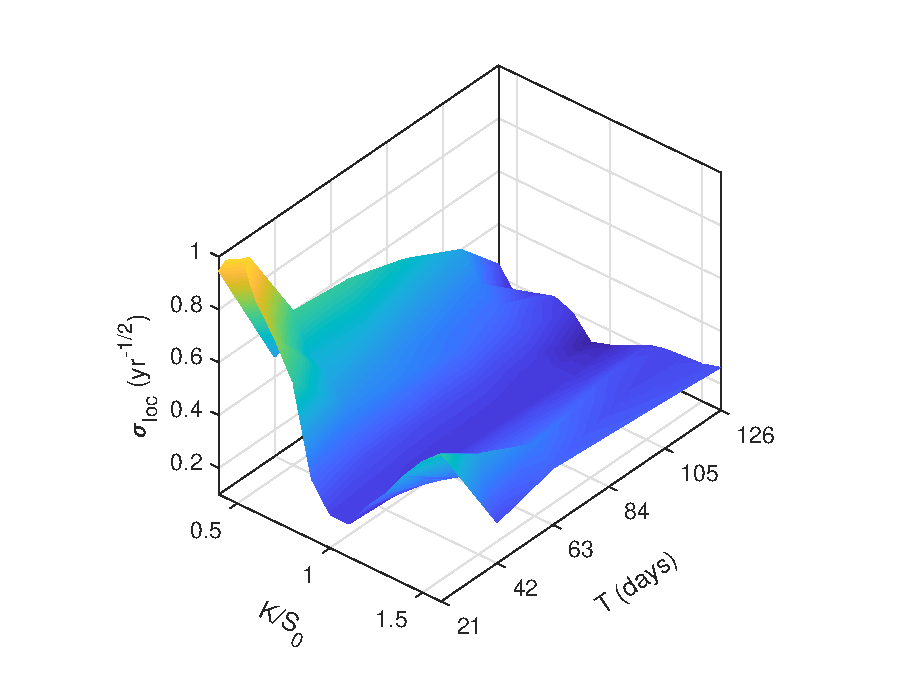
\includegraphics[width=.8\columnwidth,trim={1.7cm 0.45cm 2.cm 0.85cm},clip]{LocalV.eps}
      \caption{Local volatility surface obtained with Dupire's formula}\label{fig:DupLocVol}
    \end{figure}
    
    
Regarding now the stochastic volatility models, we calibrated them with the cost function described before using the CMA-ES optimization algorithm. The calibrated parameters for these models are represented in Tables \ref{tab:SSR}-\ref{tab:DSR}, with the resulting costs in \autoref{tab:CostsCompare}.
 
We should note that the Static SABR model was trained on data for each maturity independently, whereas the Heston and Dynamic SABR models were trained on all maturities together dependently, as an ensemble. In other words, the Static SABR model was trained 4 times (once for each maturity) on a data set of 7 implied volatilities (with different strikes), whereas Heston and Dynamic SABR were trained on a data set of 28 (7$\times$4) implied volatilities, disregarding maturity. For this reason, in \autoref{tab:CostsCompare}, for the Static SABR model we show the sum of the costs of calibration on each maturity, $\Sigma_{\mathrm{Costs}}$.

To have a benchmark for how well each model performs, we also trained a constant volatility model twice, with the calibration done independently for each maturity, as for Static SABR, and dependently, like Heston. Because the calibrated constant volatilities are not relevant for our results, they are not shown here, though we represent their costs in \autoref{tab:CostsCompare}.


\begin{table}[H]
    \centering
        \renewcommand{\arraystretch}{0.8}
\begin{tabular}{@{}lcccr@{}}
\toprule
 $T$(days) & $\alpha$($\SI{}{\year\tothe{-0.5}}$) & $\beta$ & $\rho$ & $\nu$($\SI{}{\year\tothe{-0.5}}$)  \\ \midrule
21 & 0.24 & 0.38 & -0.38 & 2.10 \\
42 & 0.24 & 0.74 & -0.37 & 1.45\\
63 & 0.24 & 0.78 & -0.31 & 1.14\\
126& 0.23 & 0.88 & -0.24 & 0.82\\
\bottomrule
\end{tabular}
  \caption{Fitted parameters for each maturity (fitted independently) under Static SABR model.}
  \label{tab:SSR}
\end{table}

\begin{table}[H]
    \centering
        \renewcommand{\arraystretch}{0.8}
\begin{tabular}{@{}lcccr@{}}
\toprule
$\kappa$($\SI{}{\year\tothe{-1}}$) & $\overline{\nu}$($\SI{}{\year\tothe{-1}}$) & $\nu_0$($\SI{}{\year\tothe{-1}}$) & $\rho$ & $\eta$($\SI{}{\year\tothe{-1}}$)  \\ \midrule
53.44 & 0.07 & 0.10 & -0.41 & 6.26  \\
\bottomrule
\end{tabular}
  \caption{Fitted parameters for all maturities (fitted simultaneously) under the Heston model.}
  \label{tab:HR}
\end{table}

\begin{table}[H]
    \centering
        \renewcommand{\arraystretch}{0.8}
\begin{tabular}{@{}lccccr@{}}
\toprule
$\alpha$($\SI{}{\year\tothe{-0.5}}$) & $\beta$ & $\rho_0$ & $a$($\SI{}{\year\tothe{-1}}$) & $\nu_0$($\SI{}{\year\tothe{-0.5}}$) & $b$($\SI{}{\year\tothe{-1}}$)  \\ \midrule
0.25 & 0.63 & -0.42 & 0 & 1.87 & 41.69 \\
\bottomrule
\end{tabular}
  \caption{Fitted parameters for all maturities (fitted simultaneously) under the Dynamic SABR model.}
  \label{tab:DSR}
\end{table}


\begin{table}[H]
    \centering
        \renewcommand{\arraystretch}{0.8}
\begin{tabular}{@{}lcr@{}}
\toprule
 Model & Cost & $\Sigma_{\mathrm{Costs}}$ \\ \midrule
Constant Vol. (indep.) & - & 0.1150 \\
Constant Vol. (dep.) & 0.1248 & - \\
Dupire & - & - \\
Static SABR & - & 0.0008 \\
Heston & 0.0025 & - \\
Dynamic SABR & 0.0108\\
\bottomrule
\end{tabular}
  \caption{Comparison between the costs from the calibrated stochastic volatility models.}
  \label{tab:CostsCompare}
\end{table} 
 
We now analyze the calibration results presented before for the stochastic volatility models.

Starting with Static SABR, we first note that the cost after calibration is extremely low, showing an improvement of $99.3\%$ over the cost of the constant volatility model (with independent fits). This seems to suggest that the model fits the data almost perfectly, though this conclusion should be taken carefully: we have an extremely small amount of data points (7 for each maturity) for the comparatively large number of parameters used (4 parameters in total). This will cause our model to overfit the data, explaining our very low costs. To further corroborate this hypothesis, we note that the parameter $\beta$, which is expected to remain constant, varies wildly between maturities.
Finally, we note that, as expected, the parameter $\rho$ is always negative and that both $\rho$ and $\nu$ seem to tend to zero with time, validating the hypothesis from Fernandez \textit{et al.}
 

Regarding now the Heston model, we first emphasize the low cost value after calibration, with an improvement of $98.0\%$ over the constant volatility model (with dependent fits), which suggests that this model fits the data very well, without the overfitting problem from Static SABR.
The parameter $\kappa$ is very large, which means that the variance process ($\nu(t)=(\sigma(t))^2$) tends to its mean value, $\overline{\nu}$, very fast and that $\nu_0$ has almost no influence. Furthermore $\rho$ is negative, as expected, and $\eta$ is very large meaning that the variance process will be quite erratic.
 
Considering the Dynamic SABR model, the improvement of the cost value over the constant volatility model (with dependent fits) is now (only) $91.3\%$.
The parameter $a$ being $0$ implies that the function $\rho(t)$ is stuck at $\rho_0$, and the parameter $b$ being very large means that $\nu(t)$ goes to $0$ extremely fast. These results are very inconsistent with what is observed in the Static SABR model, where the $\rho$ and $\nu$ tend (slowly) to zero with time. This seems to suggest that the functions chosen to model these two parameters were not appropriate.


Finally, comparing all the stochastic volatility models, we can say that even though the Static SABR model presented the lowest cost, because of the mentioned overfitting, the Heston model might be the one that performs best among the three.
 
 
 
 
 
Having trained the models we are now able to simulate the results to produce forecasts and compare the models' simulations with one another.
The simulations were performed for all four maturities mentioned before, but, due to redundancy, we only show the plots for the first maturity of 1 month.

Regarding Dupire's local volatility model, having obtained the local volatility surface we are able to simulate the stock price paths with the discretization method described before. From these, we can extract the implied volatilities for many different strikes (converting them from option prices). These simulations are performed $100$ times for each strike and then averaged to produce the \emph{simulated function}, as shown in Figure \ref{fig:Dup1}. The simulations don't always produce the exact same results and some variation might occur. To represent this variation we also show the 95\% \emph{confidence bands} of the simulations in the plot (i.e. 95\% of all observations are contained within these bands). In the same plot we also represent the implied volatility data for the first maturity.

Considering the stochastic volatility models, we show the same information as for Dupire's model but we also include the calibrated closed form solutions, which we call \emph{theoretical functions}.


To run the Monte Carlo pricers we used an initial stock price of $S_0=1\text{\euro}$, a risk-free interest rate $r=0$, a time step size $\Delta t=0.5$\ days and simulated a total of 100\ 000 paths.

\newpage
    
\begin{figure}[H]
  \begin{subfigmatrix}{1}
    \subfigure[Dupire's model]{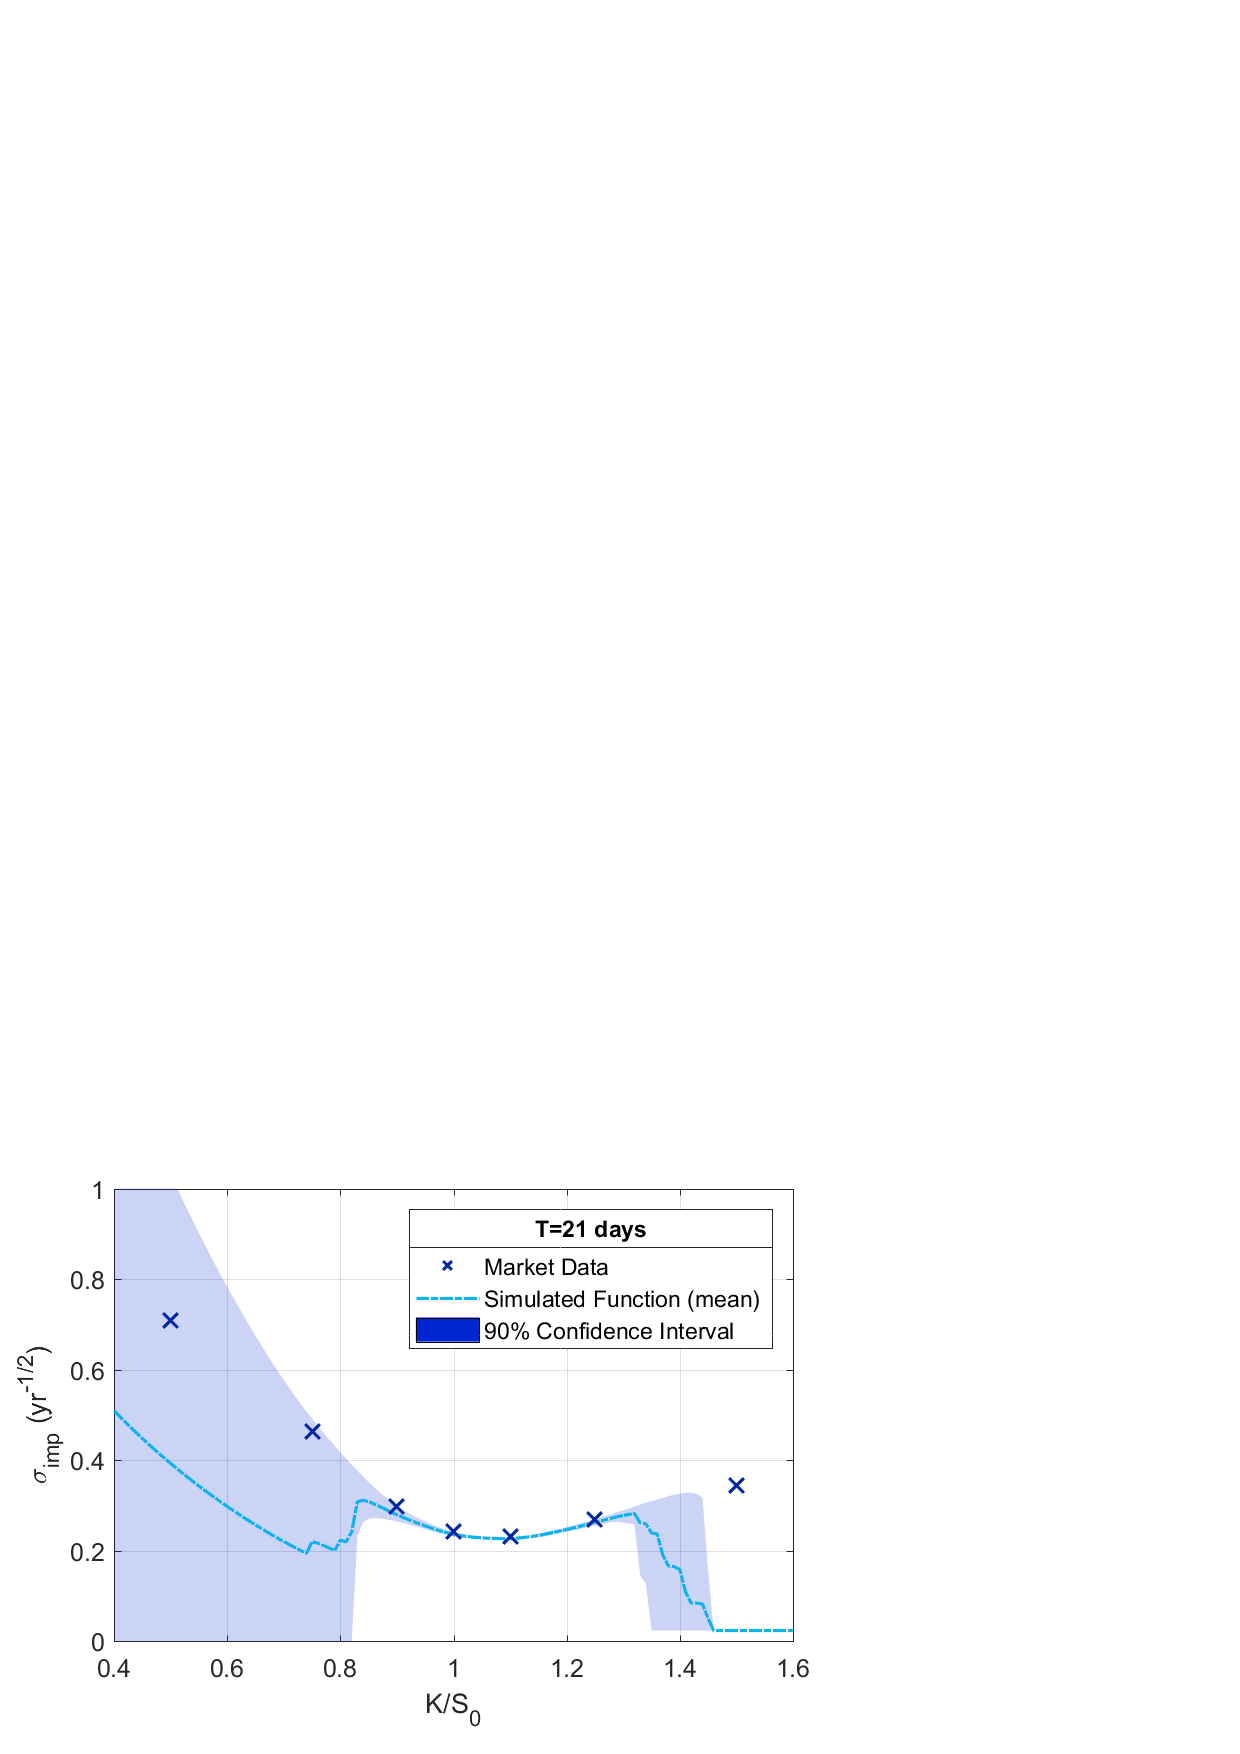
\includegraphics[width=.95\columnwidth,trim={0.25cm 0.45cm 1.1cm 1.4cm},clip]{Dup1.png}\label{fig:Dup1}}
    \subfigure[Static SABR]{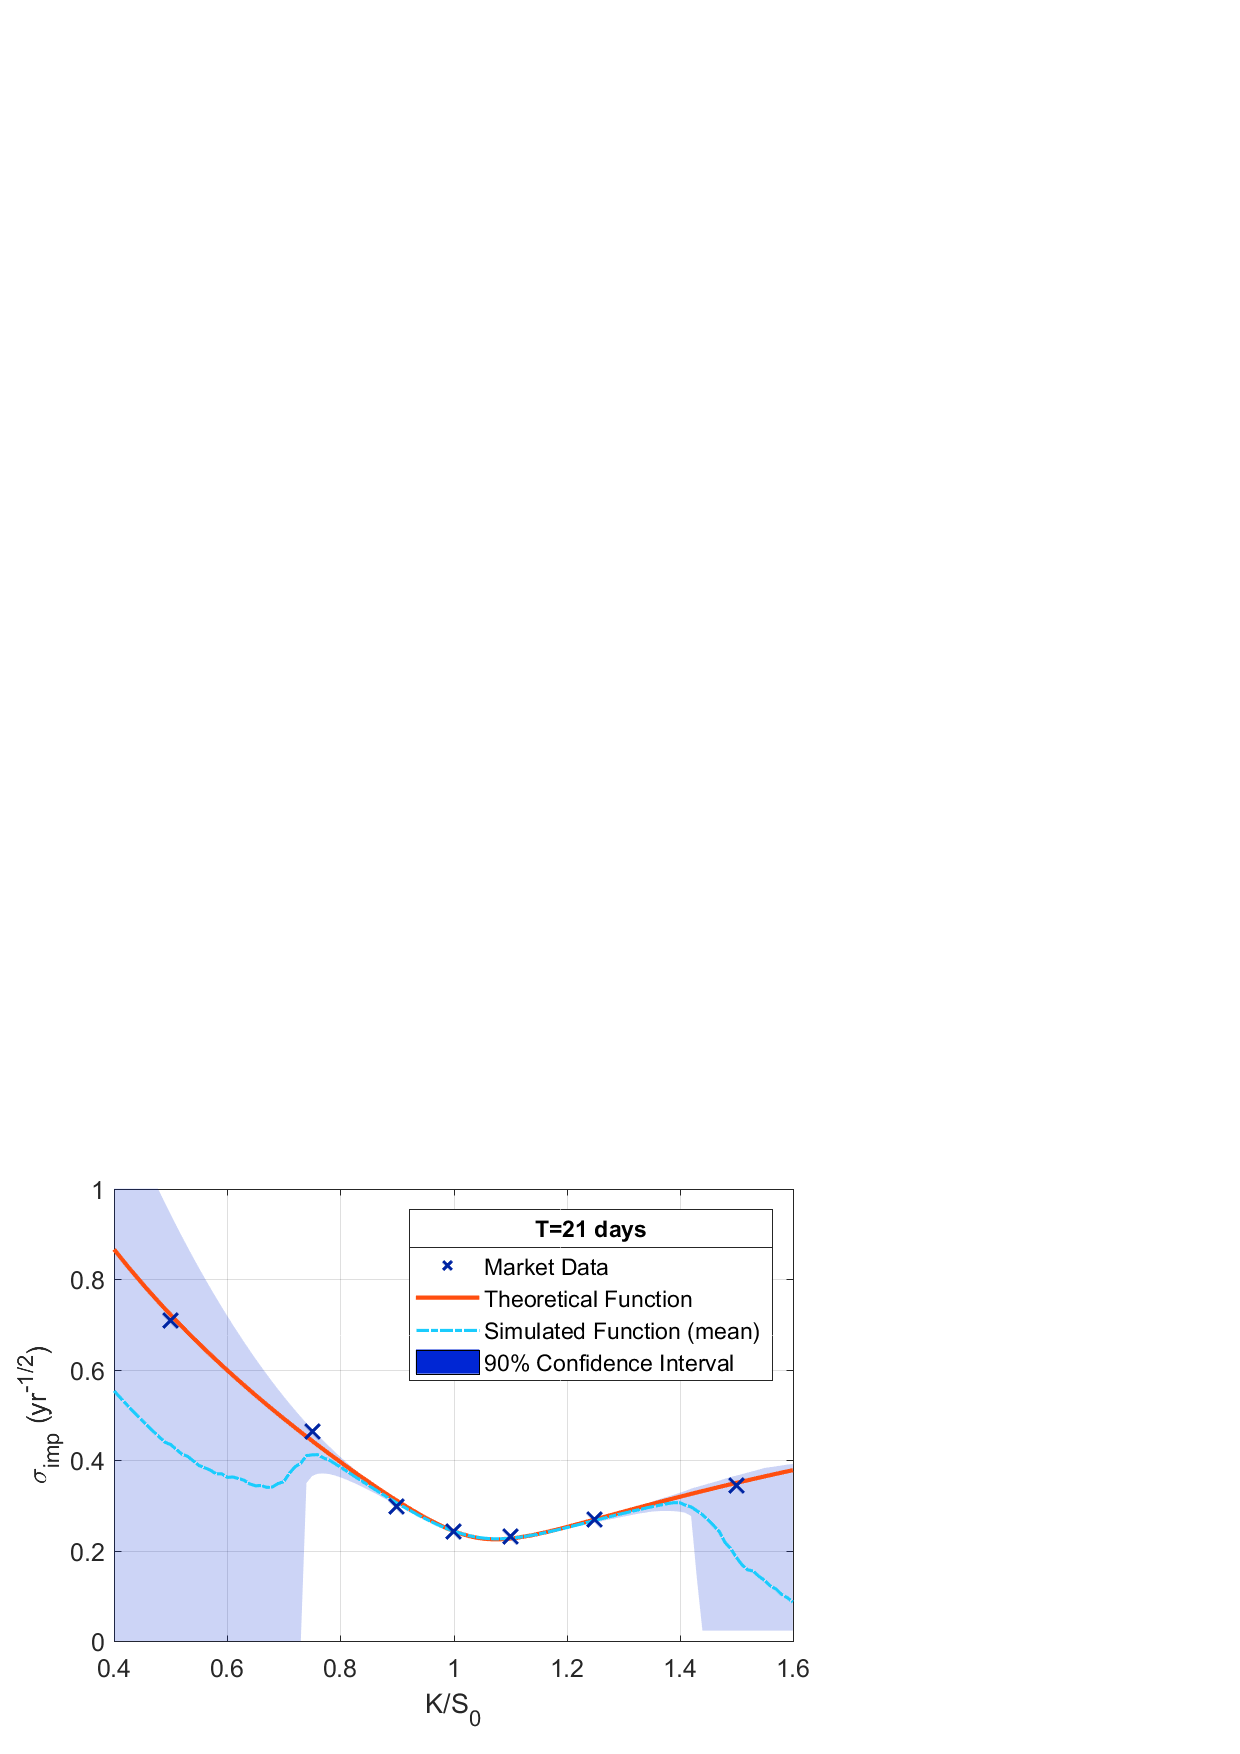
\includegraphics[width=.95\columnwidth,trim={0.25cm 0.45cm 1.1cm 1.4cm},clip]{SSABR1.png}}
    \subfigure[Heston model]{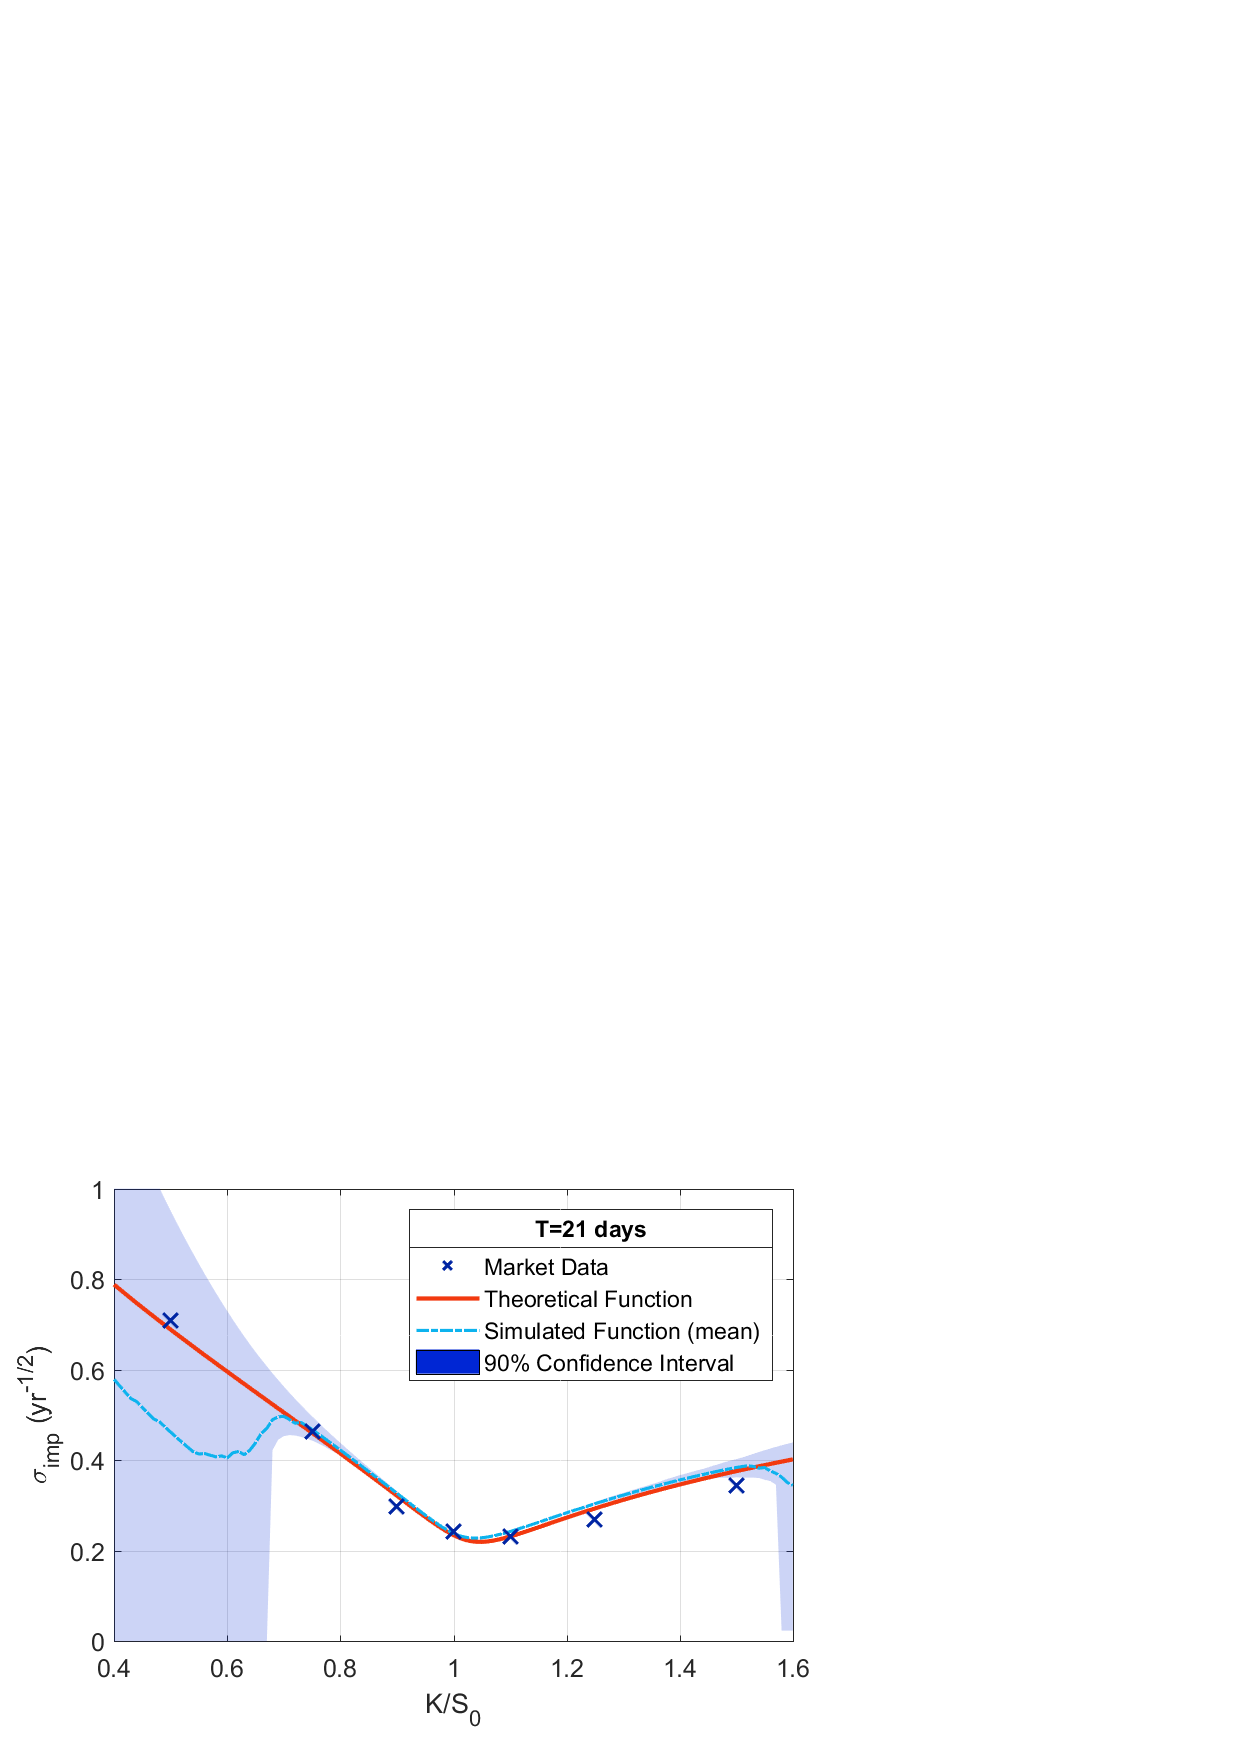
\includegraphics[width=.95\columnwidth,trim={0.25cm 0.45cm 1.1cm 1.4cm},clip]{H1.png}}
    \subfigure[Dynamic SABR]{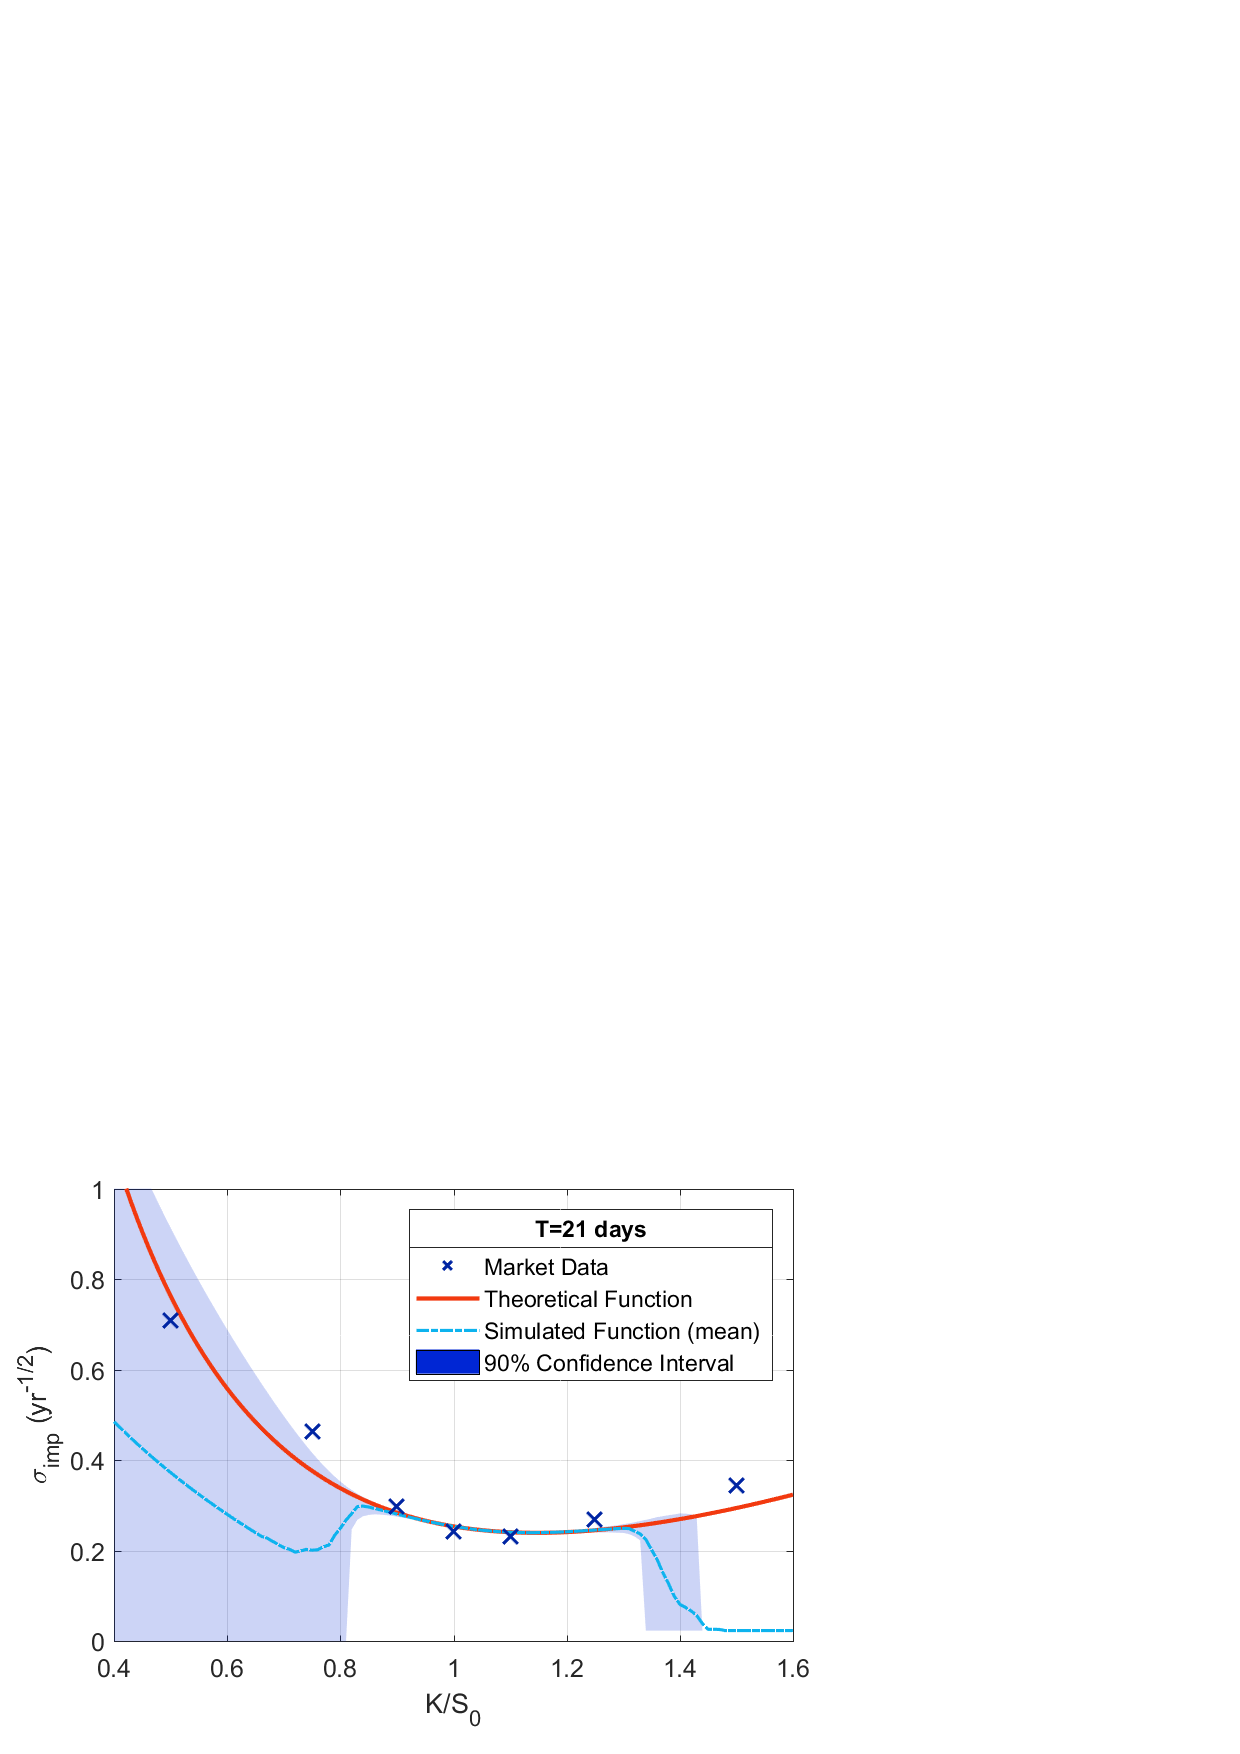
\includegraphics[width=.95\columnwidth,trim={0.25cm 0.45cm 1.1cm 1.4cm},clip]{DS1.png}}
  \end{subfigmatrix}
  \caption{Simulations and closed-form solutions under each model}
\end{figure}
    
We now analyze the results shown in the previous plots.

We begin by noting that in the regions with strikes around $S_0$ all simulations follow the closed form solutions very closely, with almost no variation, which seems to suggest that the implementation was done correctly for all models. Furthermore, all models match the implied volatility data quite well in this region.

Regarding the simulated functions, we can see that they decrease significantly for large strikes, presenting also a large variation (i.e. wide confidence bands). This can be explained by the low number of stock price paths that are able to reach such high strikes in such a short maturity, which causes the resulting option prices to be too dependent on only a few simulations, which explains the variation. If we increase the maturity or the number of simulations this phenomenon disappears, since more paths are able to reach the high strikes and contribute to the option price.


Finally, to explain the wide confidence bands for the low strikes on all models we require the concept of \emph{relative change} introduced before. We noted previously that for low strikes the implied volatility is extremely sensitive to the option price. Thus, because we are simulating option prices and only then converting them to implied volatilities, even a very slight variation in the simulations will produce a a slightly different option price which is converted into an entirely different implied volatility, justifying the wide confidence bands.

With the Monte Carlo pricers working properly, we should be able to price any options, European or not, by adapting our algorithm.
We priced several Barrier options with different barrier levels under each of the models. Due to redundancy, in \autoref{fig:BarrHest} we only represent Barrier option prices with different barrier levels using the Heston model. For comparison, we also show the prices of the corresponding European option.

\begin{figure}[H]
    \centering
      \includegraphics[width=.8\columnwidth,trim={0.5cm 0.4cm 1cm 1cm},clip]{BarrHest}
      \caption{Barrier option prices with different barrier levels and corresponding European option prices under the Heston model.}\label{fig:BarrHest}
    \end{figure}


%%%%%%%%%%%%%%%%%%%%%%%%%%%%%%%%%%%%%%%%%%%%%%%%%%%%%%%%%%%%%%%%%%%%%%
% CONCLUSIONS
%%%%%%%%%%%%%%%%%%%%%%%%%%%%%%%%%%%%%%%%%%%%%%%%%%%%%%%%%%%%%%%%%%%%%%
%%%%%%%%%%%%%%%%%%%%%%%%%%%%%%%%%%%%%%%%%%%%%%%%%%%%%%%%%%%%%%%%%%%%%%
%     File: ExtendedAbstract_concl.tex                               %
%     Tex Master: ExtendedAbstract.tex                               %
%                                                                    %
%     Author: Andre Calado Marta                                     %
%     Last modified : 27 Dez 2011                                    %
%%%%%%%%%%%%%%%%%%%%%%%%%%%%%%%%%%%%%%%%%%%%%%%%%%%%%%%%%%%%%%%%%%%%%%
% The main conclusions of the study presented in short form.
%%%%%%%%%%%%%%%%%%%%%%%%%%%%%%%%%%%%%%%%%%%%%%%%%%%%%%%%%%%%%%%%%%%%%%

\section{Conclusions}
\label{sec:concl}
Volatility is one of the most important subjects in all of quantitative finance, due not only to its impact on the prices of options but also to its elusiveness. In this thesis we studied some of the models most used to forecast this variable.

We began by studying Dupire's local volatility model as well as Heston and Static/Dynamic SABR stochastic volatility models. We used some real implied volatility data to train the models: we generated the local volatility surface for Dupire's model and calibrated all the parameters for the stochastic volatility models using their closed form solutions.
From this calibration we concluded that the Static SABR model best fit the data, though some overfitting is expected to have occurred, for which reason we consider the Heston model to perform best. All models vastly outperform the constant volatility model.

Having trained all models, we input them into a numerical pricer, using the Monte Carlo method to estimate the option prices under each model. All simulations followed the data very closely for options with strikes around $S_0$, though some significant variation was found in the results for very low strikes and for high strikes with early maturities. In these cases great care should be employed when using these models.

Finally, we adapted our Monte Carlo pricers to price Barrier options and observed that the option prices decreased when we increased the barrier levels and remained strictly below the corresponding European option prices. Both observations were expected.

Regarding future work, one clear possibility is to improve the Monte Carlo pricer, using, for example, importance sampling or the antithetic variates method. Some different functions for $\rho(t)$ and $\nu(t)$ could also be considered, besides the ones we used.

%%%%%%%%%%%%%%%%%%%%%%%%%%%%%%%%%%%%%%%%%%%%%%%%%%%%%%%%%%%%%%%%%%%%%%
% ACKNOWLEDGMENTS
%%%%%%%%%%%%%%%%%%%%%%%%%%%%%%%%%%%%%%%%%%%%%%%%%%%%%%%%%%%%%%%%%%%%%%
%%%%%%%%%%%%%%%%%%%%%%%%%%%%%%%%%%%%%%%%%%%%%%%%%%%%%%%%%%%%%%%%%%%%%%
%     File: ExtendedAbstract_ackno.tex                               %
%     Tex Master: ExtendedAbstract.tex                               %
%                                                                    %
%     Author: Andre Calado Marta                                     %
%     Last modified : 27 Dez 2011                                    %
%%%%%%%%%%%%%%%%%%%%%%%%%%%%%%%%%%%%%%%%%%%%%%%%%%%%%%%%%%%%%%%%%%%%%%
% Acknowledge persons and institutions that supported this work.
%%%%%%%%%%%%%%%%%%%%%%%%%%%%%%%%%%%%%%%%%%%%%%%%%%%%%%%%%%%%%%%%%%%%%%

\section*{Acknowledgements}
I would like to thank Claude Cochet and both my advisors, Prof. Cláudia Philippart and Prof. Rui Dilão, for all their help and guidance and without whom this work would not have been possible. A special word of appreciation also for my family, my girlfriend and my friends for all their support.



%%%%%%%%%%%%%%%%%%%%%%%%%%%%%%%%%%%%%%%%%%%%%%%%%%%%%%%%%%%%%%%%%%%%%%
% REFERENCES
%%%%%%%%%%%%%%%%%%%%%%%%%%%%%%%%%%%%%%%%%%%%%%%%%%%%%%%%%%%%%%%%%%%%%%

% Produces the bibliography section when processed by BibTeX
%
% Bibliography style
% > entries ordered alphabetically
%\bibliographystyle{plain}
% > unsorted with entries appearing in the order in which the citations appear.
%\bibliographystyle{unsrt}
% > entries ordered alphabetically, with first names and names of journals and months abbreviated
%\bibliographystyle{abbrv}
% > entries ordered alphabetically, with reference markers based on authors' initials and publication year
%\bibliographystyle{alpha}
\bibliographystyle{abbrvnat}
% External bibliography database file in the BibTeX format (ExtendedAbstract_ref_db.bib)
\bibliography{ExtendedAbstract_ref_db}

%%%%%%%%%%%%%%%%%%%%%%%%%%%%%%%%%%%%%%%%%%%%%%%%%%%%%%%%%%%%%%%%%%%%%%
\end{document}
%%%%%%%%%%%%%%%%%%%%%%%%%%%%%%%%%%%%%%%%%%%%%%%%%%%%%%%%%%%%%%%%%%%%%%

